% !TEX root = ../main.tex
\ulfgchapter{7}{Real-Data External Validation}{chp:realdata}

\section{The question, and how the transfer test was set up}
\label{sec:r7intro}

Every result in Chapters~\ref{chp:synthetic} and~\ref{chp:attribution} came from a single
simulator. Training, validation and held-out test splits were generated by the same code from the
same signal model, differing only in random seed and in the scenarios they sample. A held-out split
of that kind shows the detector generalises to \emph{new samples} of its own domain. It cannot show
that the detector generalises to a \emph{different} domain, and no quantity of additional synthetic
data can close that gap.

This chapter therefore asks a single question:

\begin{quote}
Do the already-frozen TinyCNN and classical CFAR detectors transfer zero-shot from the synthetic
development domain to real automotive radar data?
\end{quote}

\emph{Zero-shot} here means that neither detector is retrained, fine-tuned or recalibrated against
real data. The detector weights, the input preprocessing, the CFAR window geometry and the
suppression radius all remain exactly as frozen in Chapter~\ref{chp:detectors}.

\paragraph{The operating point is the one thing that cannot carry over.}
Chapter~\ref{chp:synthetic} sets each detector's threshold by sweeping it per condition and
comparing the arms where their \emph{measured} false-alarm rates agree. That rule needs labels on
the data being scored, and CARRADA provides no false-alarm axis to sweep against. For real data the
threshold is therefore \textbf{fixed in advance: one value per frozen seed, derived from synthetic
validation data alone}. No CARRADA data of any split enters that derivation. The two chapters use
different operating-point protocols, and their headline numbers are never pooled --- a distinction
Section~\ref{sec:r7protocol} makes precise.

\paragraph{What was fixed before the evaluation, and what was revised afterwards.}
This evaluation was run at the end of the project by the person who produced the synthetic result,
knowing what that result was. The complete protocol --- ground truth, eligibility, matching,
metrics, the statistical plan, and the wording permitted for unmatched detections --- was therefore
written down and frozen \emph{before any real detector output existed}, and the real-data work ran
in a directory that reads the frozen benchmark and writes nothing back to it. Implementation and
debugging used the CARRADA \emph{training} sequences only; the validation sequences were not used at
all in this chapter.

One qualification belongs with that. The results below come from a \textbf{re-run}. The suppression
radius was later reselected on synthetic development data, and the same test sequences were scored
once more under the revised rule. No detector changed and no real measurement informed the revision,
so the result remains zero-shot as defined above --- but it is not the original untouched read.
Appendix~\ref{app:prereg} states what changed and what did not.

\paragraph{Scope.} This is an \textbf{external validation}, not a replacement for the synthetic
benchmark: a poor real-data outcome bounds the external validity of the synthetic findings rather
than retracting them. The two experiments also do not share a headline metric --- the synthetic
benchmark scores a point target within a $\pm 1$-bin gate at a matched measured false-alarm rate,
while the real dataset annotates extended regions and supports no false-alarm measurement at all.
Numbers from the two domains are never pooled anywhere in this report.

\section{CARRADA and the real-data evaluation protocol}
\label{sec:r7protocol}

\subsection{The dataset}
\label{sec:carrada}

CARRADA~\cite{ouaknine2021carrada} is a public dataset of synchronised camera and automotive radar
recordings, collected on a test track with a \SI{77}{\giga\hertz} FMCW sensor and released with
annotations on both range--angle and range--Doppler representations. It was selected for three
reasons: it publishes range--Doppler data directly, so no re-processing from raw ADC samples is
required; its annotations are given in range--Doppler coordinates, so no projection step is needed;
and its published grid geometry matches the geometry this project's simulator was configured to
reproduce.

That last point requires care. The simulator was specified in Chapter~\ref{chp:simulator} to
reproduce CARRADA's \emph{published range--Doppler grid} --- map dimensions and bin spacings --- so
that a target occupies a comparable number of cells in both domains. It does not reproduce
CARRADA's waveform, its scenes, its clutter statistics or its sensor hardware. \textbf{Matching a
grid is not matching a radar}: the geometric correspondence removes one confound, and
Section~\ref{sec:r7audit} measures how far apart the domains remain.

The dataset holds \CarradaSequences{} sequences and \CarradaFrames{} range--Doppler frames, of
which \CarradaAnnotatedFrames{} contain at least one annotated object. Two counts must be kept
apart, because they act as denominators for everything reported later. A single physical vehicle
tracked across two hundred frames contributes \emph{one} track but \emph{two hundred} frame-level
object instances: the dataset holds \CarradaObjectFrames{} frame-level object instances drawn from
only \CarradaTracks{} distinct tracks. Detection statistics are computed per frame-level instance,
but \CarradaTracks{} objects across \CarradaSequences{} sequences is a small amount of genuinely
independent content, which is why the statistical treatment takes the \emph{sequence} --- not the
frame or the object --- as its unit of analysis.

Objects belong to three classes --- pedestrian, cyclist and car --- and no frame contains more than
two annotated objects. The dataset therefore offers no counterpart to the multi-target,
mutual-masking and unresolved-pair conditions that Chapter~\ref{chp:synthetic} used to separate
detector behaviour; that limitation is revisited in Section~\ref{sec:limits}.

CARRADA publishes a sequence-level partition, reproduced in Table~\ref{tab:carrada_splits}, and this
work adopts it unchanged. Splitting instead by frame would be indefensible here: with only
\CarradaTracks{} tracks, consecutive frames of the same object are near-duplicates, and a random
frame-level split would place the same physical vehicle on both sides of the partition. The reported
test performance would then be closer to a memorisation check than to a generalisation measurement.
Only the test split is scored in this chapter.

\begin{table}[H]
\centering
\caption{Official CARRADA sequence-level splits, used unchanged.}
\label{tab:carrada_splits}
\begin{tabular}{@{}lrrrr@{}}
\toprule
\textbf{Split} & \textbf{Sequences} & \textbf{Frames} & \textbf{Annotated} & \textbf{Object instances} \\
\midrule
Train                  & \CarradaTrainSeq & \CarradaTrainFrames & 4,319 & \CarradaTrainObjects \\
Validation             & \CarradaValSeq   & \CarradaValFrames   & 1,483 & \CarradaValObjects \\
\textbf{Test}          & \CarradaTestSeq  & \CarradaTestFrames  & 1,391 & \CarradaTestObjects \\
\bottomrule
\end{tabular}
\end{table}

\subsection{Feeding the frozen detectors real data}

Two checks were needed before either detector could be run, and both were passed without modifying
any detector.

\textbf{The representation transfers.} CARRADA publishes more than one numerical representation of
each range--Doppler frame. A cross-check over 240 frames confirmed that the published decibel array
is consistent with a logarithmic representation of the radar amplitude/power
data.\footnote{Regressing the logarithm of one representation against another gives a slope of
\RzeroSlope{} $\pm$ \RzeroSlopeSD{} with a residual standard deviation of \RzeroResidual{}\,dB and
no dependence on signal level or map position --- the signature of a $20\log_{10}$ transform.} This
is sufficient for both detectors: CFAR uses power ratios, so an unknown constant scale cancels,
while TinyCNN subtracts the frame-median level during preprocessing, which removes the same
constant. Absolute sensor calibration is therefore not required, and \textbf{no detector-specific
preprocessing was redesigned for real data}: both arms run the code they were frozen with.

\textbf{The grid transfers exactly.} Every one of the \CarradaFrames{} frames is a
$256 \times 64$ array matching the simulator's map dimensions, and the annotation coordinates index
that array directly. No resampling, interpolation or coordinate transformation is required anywhere
in the pipeline.

\subsection{Why the synthetic metric cannot be reused}

One difference forces a new metric. A synthetic target occupies a single true cell, and
Chapter~\ref{chp:detectors} scores detections against it with a $\pm 1$-bin gate. CARRADA annotates
\emph{extended object support}: a segmentation region covering tens of cells, whose median extent is
$18 \times 13$ bins for a car, $11 \times 11$ for a cyclist and $9 \times 9$ for a pedestrian
(Figure~\ref{fig:r0_footprint} in Appendix~\ref{app:tables}). There is no point target to match
within $\pm 1$ bin, and inventing one --- by taking a centroid, a box centre or the brightest cell
inside the mask --- would mean scoring the detectors against a construct of this project rather than
an annotation the dataset provides.

\subsection{The protocol}

Redesigning a metric with results in view is exactly where unconscious bias operates, so the
protocol was written in full and frozen before any real detector output existed.
Table~\ref{tab:prereg} summarises what it fixes.

\begin{table}[H]
\centering
\caption{The real-data evaluation protocol, fixed before any real detector output existed.}
\label{tab:prereg}
\begin{tabular}{@{}p{0.26\textwidth}p{0.65\textwidth}@{}}
\toprule
\textbf{Element} & \textbf{Decision} \\
\midrule
Ground truth & The dense segmentation support. No point target is invented; centroid, box centre,
brightest cell and sparse centroid are all explicitly rejected. \\
Eligible region & The frozen $21\times 9$ detector-valid interior, unchanged from
Chapter~\ref{chp:detectors}. \\
Eligible object & One whose support intersects that region in at least one cell. \\
Matching & One-to-one, maximum-cardinality, identical code for every detector arm. \\
Primary metric & Exact dense-mask object recall: the fraction of eligible objects for which an
assigned peak lies inside the annotated support. \\
Tolerance analysis & The same recall with the mask dilated by $\pm 1$ and $\pm 3$ bins. \\
Localisation & \textbf{Not reported.} CARRADA supplies no point truth. \\
False alarms & \textbf{Not reported as $P_{fa}$}, in any form. \\
Burden metric & Unmatched detections per frame. \\
Statistics & Paired bootstrap over the \RoneNseq{} test sequences, 10{,}000 replicates. Seed
variability reported separately and never merged with sequence variability. \\
Primary classical arm & CA-CFAR. \\
\bottomrule
\end{tabular}
\end{table}

Two entries deserve explanation, because they are where this evaluation departs most sharply from
Chapter~\ref{chp:synthetic}.

\paragraph{Why no false-alarm rate is reported.} A false-alarm measurement requires knowing that a
detection corresponds to nothing real. CARRADA annotates only its \CarradaTracks{} tracked road
users; it does not annotate the buildings, parked vehicles, poles and roadside structure that a real
scene contains, and bright unannotated returns occur in a measurable fraction of frames. A peak
outside every annotated mask may therefore be infrastructure, static clutter, multipath, an
unannotated object --- or a genuine false alarm, with no way to distinguish them. Reporting such
counts as $P_{fa}$ would assert knowledge the dataset does not contain. They are reported instead as
\emph{unmatched detections per frame}, an output-density measure, and that term is used consistently
throughout.

\paragraph{Why the operating point is a different protocol.} Within each experiment in this thesis
all detector arms share the same evaluation rule and operating-point definition. Across domains they
cannot. Chapter~\ref{chp:synthetic} sweeps each detector's score threshold \emph{per condition} and
compares the arms where their measured false-alarm rates agree --- an \textbf{evaluation operating
point}, not a deployable setting, whose purpose is to remove threshold choice as a confound. This
chapter has no false-alarm axis to sweep against, so a \textbf{single global threshold} was derived
per frozen seed from \emph{synthetic validation data alone}, pooled across all eight scenario
conditions at a measured per-cell false-alarm rate of $10^{-4}$, and applied unchanged to every real
frame. That is the harder of the two requirements: one fixed threshold, chosen without sight of the
data it will run on. The consequence, fixed in advance, is that the two chapters' headline numbers
are \textbf{not poolable}.

\section{Zero-shot transfer: the result}
\label{sec:r1}

The official test sequences were scored under the protocol above --- once in the original read, and
once again in the disclosed re-run at the revised suppression radius, which is what is reported
here. All eight frozen network seeds and all four CFAR variants were evaluated on the same
\CarradaTestFrames{} frames. Of the \CarradaTestObjects{} object instances in the test split,
\RoneEligibleObjects{} remain eligible once the detector-valid interior is applied; the difference is
a single instance whose support lies entirely in the excluded border.

\begin{table}[H]
\centering
\caption{Exact dense-mask object recall on the held-out CARRADA test split, over
\RoneEligibleObjects{} eligible object instances.}
\label{tab:r1_primary}
\begin{tabular}{@{}lc@{}}
\toprule
\textbf{Detector} & \textbf{Exact dense-mask object recall} \\
\midrule
Frozen CA-CFAR (primary classical arm) & \textbf{\RoneCFARCA} \\
Frozen TinyCNN (mean over 8 seeds)     & \textbf{\RoneTinyCNN} \\
\midrule
Pooled difference, TinyCNN $-$ CA-CFAR           & \RonePooledDelta \\
Sequence-balanced paired difference               & \textbf{\RoneDelta} \\
95\,\% confidence interval on that difference     & $[\RoneCIlo,\ \RoneCIhi]$ --- includes zero \\
\bottomrule
\end{tabular}
\end{table}

\textbf{At exact annotated support the two arms are statistically indistinguishable.} The
sequence-balanced difference of \RoneDelta{} carries a \SI{95}{\percent} confidence interval of
$[\RoneCIlo,\ \RoneCIhi]$, which includes zero. The point estimate favours the classical detector and
CA-CFAR is ahead in \RoneSeqCFARLead{} of the \RoneNseq{} test sequences, but the margins are small
and the network leads in the remaining one. The interval does not license a claim that either arm
wins. \textbf{The synthetic ordering is not reproduced on real data, and it is not cleanly reversed
either: it disappears.}

The raw pooled recall difference is \RonePooledDelta{} when all eligible objects are counted
together. For statistical inference, the sequence-balanced estimate is \RoneDelta{}, which gives
each of the \RoneNseq{} test sequences equal weight so that a long sequence cannot dominate the
result. Confidence intervals and conclusions therefore use the sequence-balanced estimate.

The second half of the result is on a different axis. \textbf{At their frozen operating points the
network emits \RoneBurdenRatio{} times CA-CFAR's unmatched output} for statistically
indistinguishable exact recall: \RoneBurdenTinyCNN{} unmatched detections per frame against
\RoneBurdenCFARCA{} (Table~\ref{tab:r1_burden}).

\begin{table}[H]
\centering
\caption{Unmatched detections per frame beside exact recall. This is an output-density measure and
\textbf{not} a false-alarm rate.}
\label{tab:r1_burden}
\begin{tabular}{@{}lcc@{}}
\toprule
\textbf{Detector} & \textbf{Unmatched detections / frame} & \textbf{Exact recall} \\
\midrule
CA-CFAR & \RoneBurdenCFARCA & \RoneCFARCA \\
TinyCNN & \RoneBurdenTinyCNN & \RoneTinyCNN \\
GO-CFAR & \RoneBurdenCFARGO & \RoneCFARGO \\
SO-CFAR & \RoneBurdenCFARSO & \RoneCFARSO \\
OS-CFAR & \RoneBurdenCFAROS & \RoneCFAROS \\
\bottomrule
\end{tabular}
\end{table}

The secondary CFAR variants are important to the interpretation. GO-CFAR reaches \RoneCFARGO{}
recall, SO-CFAR \RoneCFARSO{} and OS-CFAR \RoneCFAROS{}, all above the frozen TinyCNN's
\RoneTinyCNN{}. Their higher recall comes with substantially higher unmatched output, around
\RoneBurdenCFARGO{}--\RoneBurdenCFAROS{} detections per frame rather than TinyCNN's
\RoneBurdenTinyCNN{} and CA-CFAR's \RoneBurdenCFARCA{}. Thus the zero-shot TinyCNN does not dominate
the classical family: several CFAR variants achieve substantially higher raw recall, albeit at
greater output burden. \textbf{On this dataset recall and output density move together for every
detector tested}, which is precisely why recall alone cannot rank them. CA remains the primary
comparator as fixed in advance; no variant was promoted after the fact.

\begin{figure}[H]
\centering
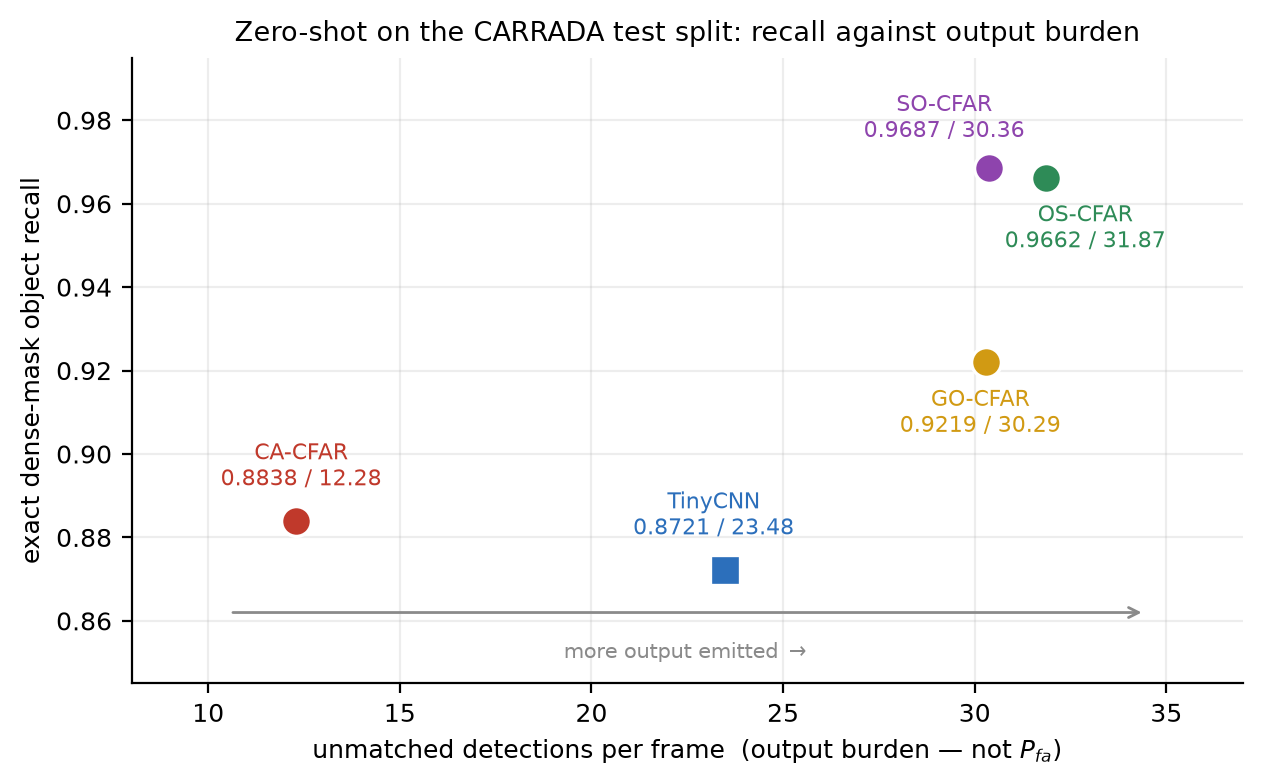
\includegraphics[width=0.88\textwidth]{figures/Chapter7/ch7_fig_alldetector.png}
\caption[All detector arms on the CARRADA test split]{The robust CFAR variants achieve the highest
raw recall, while CA-CFAR gives the lowest output burden. TinyCNN lies between these regimes and
does not dominate the classical family under zero-shot transfer. Each point is one detector at its
frozen operating point; labels give recall and unmatched detections per frame.}
\label{fig:alldetector}
\end{figure}

\begin{figure}[htbp]
\centering
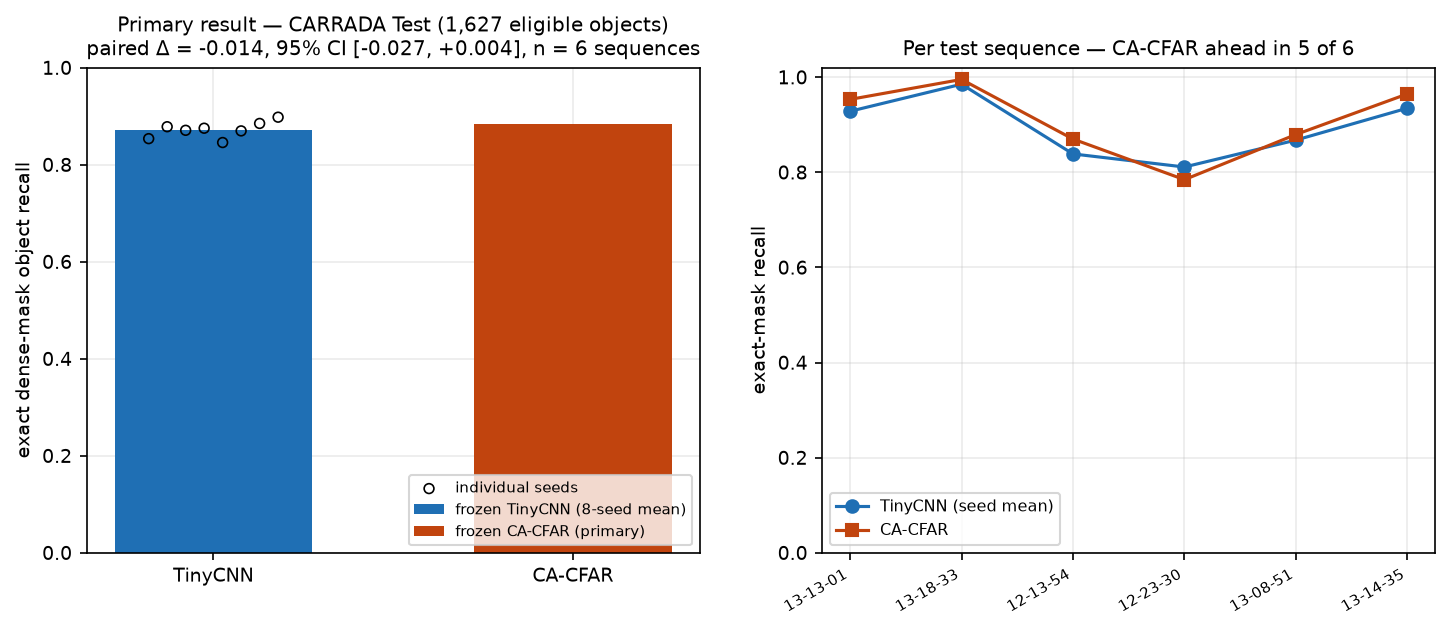
\includegraphics[width=\textwidth]{figures/Chapter7/r1_fig1_primary_and_per_sequence.png}
\caption[Primary real-data result and per-sequence breakdown]{The synthetic ordering does not carry
to real data. Left: exact dense-mask object recall, with the eight individual network seeds
overlaid. Right: the same comparison per test sequence --- CA-CFAR ahead in \RoneSeqCFARLead{} of
\RoneNseq{} sequences, the network in the remaining one, all six margins small.}
\label{fig:r1_primary}
\end{figure}

Three cautions belong with the burden column, and they are the reason it must not be read as a
false-alarm rate. The annotation covers only tracked road users. The suppression window is sized for
point targets: a $\ProtocolNmsWin \times \ProtocolNmsWin$ window is far smaller than a median car's
$18 \times 13$ support, so one real object can legitimately produce several surviving peaks --- which
occurs for \RoneMultiPeakTinyCNN{} of objects for the network and \RoneMultiPeakCFARCA{} for
CA-CFAR, of which one-to-one matching credits exactly one. And the extra output is not generated by
the annotated objects: the network averages \RoneBurdenTinyCNNAnn{} unmatched detections on
annotated frames against \RoneBurdenTinyCNNEmpty{} on annotation-empty ones, and CA-CFAR
\RoneBurdenCFARCAAnn{} against \RoneBurdenCFARCAEmpty{}. Output density is a property of the scene,
not of the annotation --- which is exactly why CARRADA cannot price it.

\section{Why the synthetic advantage disappeared}
\label{sec:r7audit}

Before either detector was run on real data, the two domains were compared directly, so that
whatever the detectors then did could be read against a measured baseline rather than an assumption.
No detector was involved in any measurement in this section. Its purpose here is to explain the
result above and to motivate the interventions of Chapter~\ref{chp:domaingap}.

To compare background statistics fairly, the same background mask was used in both domains. Cells
were excluded if they were close to an annotated target, inside the strong zero-Doppler ridge, or
inside the border where the $21 \times 9$ detector window cannot operate ($\pm 3$-bin target
dilation and $\pm 4$-bin zero-Doppler exclusion, leaving the same
$236 \times 56 = 13{,}216$ cells the detectors themselves see). Statistics were then computed only
from the remaining background cells, with no percentile trimming at any point. Uncertainty was
measured across independent groups --- CARRADA sequences and simulator conditions --- rather than
treating neighbouring frames or millions of correlated cells as independent samples.

\begin{table}[H]
\centering
\caption{Background statistics, measured on the same eligible population in both domains with no
trimming. Uncertainty is across groups, not frames.}
\label{tab:r0_stats}
\small
\begin{tabular}{@{}lccc@{}}
\toprule
\textbf{Statistic} & \textbf{CARRADA} & \textbf{Simulator} & \textbf{Ideal} \\
\midrule
Coefficient of variation, $CV(P)$ & \RzeroCarradaCV{} $\pm$ \RzeroCarradaCVSE{} & \RzeroSimCV{} $\pm$ \RzeroSimCVSE{} & 1.000 \\
Effective Gamma shape, $k$        & \RzeroCarradaGammaK{} $\pm$ \RzeroCarradaGammaKSE{} & \RzeroSimGammaK{} $\pm$ \RzeroSimGammaKSE{} & 1.00 \\
Background std.\ deviation [dB]  & \RzeroCarradaDBstd{} $\pm$ \RzeroCarradaDBstdSE{} & \RzeroSimDBstd{} $\pm$ \RzeroSimDBstdSE{} & 5.57 \\
Lag-1 correlation, range axis     & \RzeroCarradaLagRange{} $\pm$ \RzeroCarradaLagRangeSE{} & \RzeroSimLagRange{} $\pm$ \RzeroSimLagRangeSE{} & --- \\
Lag-1 correlation, Doppler axis   & \RzeroCarradaLagDoppler{} $\pm$ \RzeroCarradaLagDopplerSE{} & \RzeroSimLagDoppler{} $\pm$ \RzeroSimLagDopplerSE{} & --- \\
\bottomrule
\end{tabular}
\end{table}

Four readings follow, and they are the four differences that Chapter~\ref{chp:domaingap} acts on.

\paragraph{The simulator behaves exactly as designed.} Its background has $k = \RzeroSimGammaK{}$
against a theoretical value of 1.0 for single-look exponential speckle, and a decibel spread of
\RzeroSimDBstd{}\,dB against a theoretical 5.57\,dB, uniformly across range. This is an independent
validation of the clutter model of Chapter~\ref{chp:simulator}, obtained as a by-product of building
the comparison.

\paragraph{CARRADA is markedly smoother.} Its effective Gamma shape is $k = \RzeroCarradaGammaK{}$
and its decibel spread \RzeroCarradaDBstd{}\,dB, less than half the simulator's. The wording is
deliberate: the measurement licenses the statement that CARRADA background statistics are consistent
with an \emph{effective Gamma shape} near \RzeroCarradaGammaK{}. It does not license a claim that the
sensor performs some number of independent looks, which the dataset authors document nowhere.

\paragraph{Smoother does not mean cleaner.} Lower cell-to-cell fluctuation is not less clutter. The
same audit finds CARRADA carrying far stronger \emph{localised} structure --- a zero-Doppler ridge of
\RzeroCarradaRidge{}\,dB with a half-width of only $\pm\RzeroCarradaRidgeHalf{}$ bin, against the
simulator's broader and weaker \RzeroSimRidge{}\,dB spread over $\pm\RzeroSimRidgeHalf{}$ bins
(Figure~\ref{fig:r0_ridge}). The real domain is \emph{different}, not simply easier or harder: a
flatter field interrupted by strong narrow structure, rather than a uniformly grainy one.

\paragraph{CARRADA is not stationary in range.} Measured over the same fixed blocks used throughout
this chapter, its effective Gamma shape varies by roughly a factor of two and a half between the
nearest and the middle blocks. The simulator's is flat across every block. A detector tuned on a
stationary background therefore meets, in the real domain, a field whose statistics change with
range.

One residual mismatch is recorded alongside these because Chapter~\ref{chp:domaingap} does
\emph{not} correct it: the lag-1 Doppler correlations differ sharply between the domains
(\RzeroCarradaLagDoppler{} against \RzeroSimLagDoppler{}), while the range correlations are
statistically indistinguishable.

\begin{figure}[htbp]
\centering
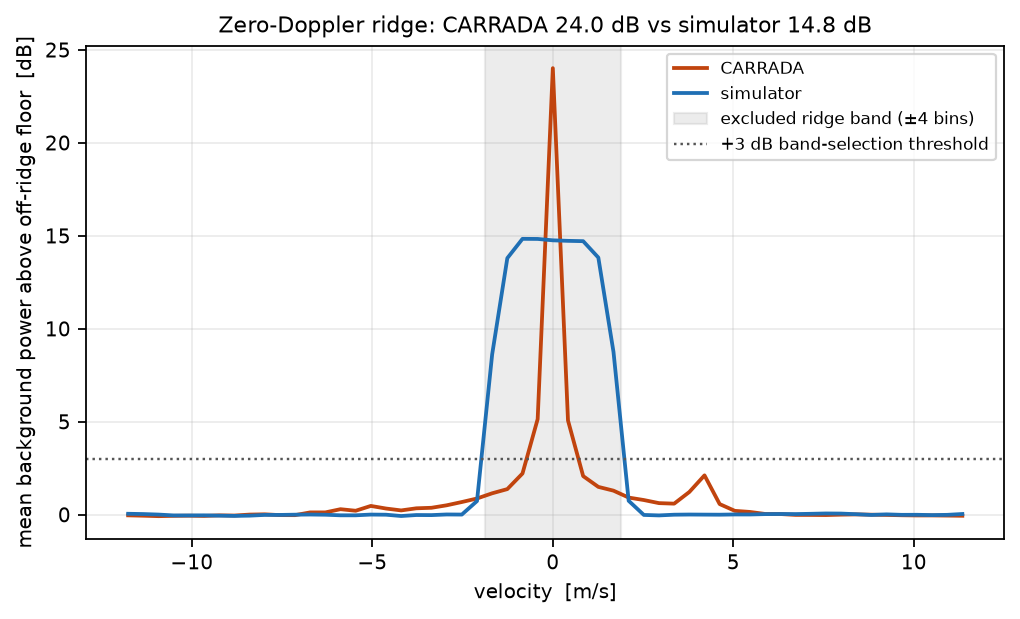
\includegraphics[width=0.85\textwidth]{figures/Chapter7/r0_fig4_zero_doppler_ridge.png}
\caption[Zero-Doppler ridge profiles]{The largest single structural difference between the domains:
CARRADA's zero-Doppler ridge is narrow and intense, the simulator's broad and weak. The shaded band
is the region excluded from the background statistics of Table~\ref{tab:r0_stats}.}
\label{fig:r0_ridge}
\end{figure}

Figure~\ref{fig:rd_domains} shows one frame from each domain on identical axes, to make the
measured differences visible. It is included for intuition and is explicitly not evidence: it shows
two hand-picked frames, whereas Table~\ref{tab:r0_stats} measures every frame in both domains.

\begin{figure}[htbp]
\centering
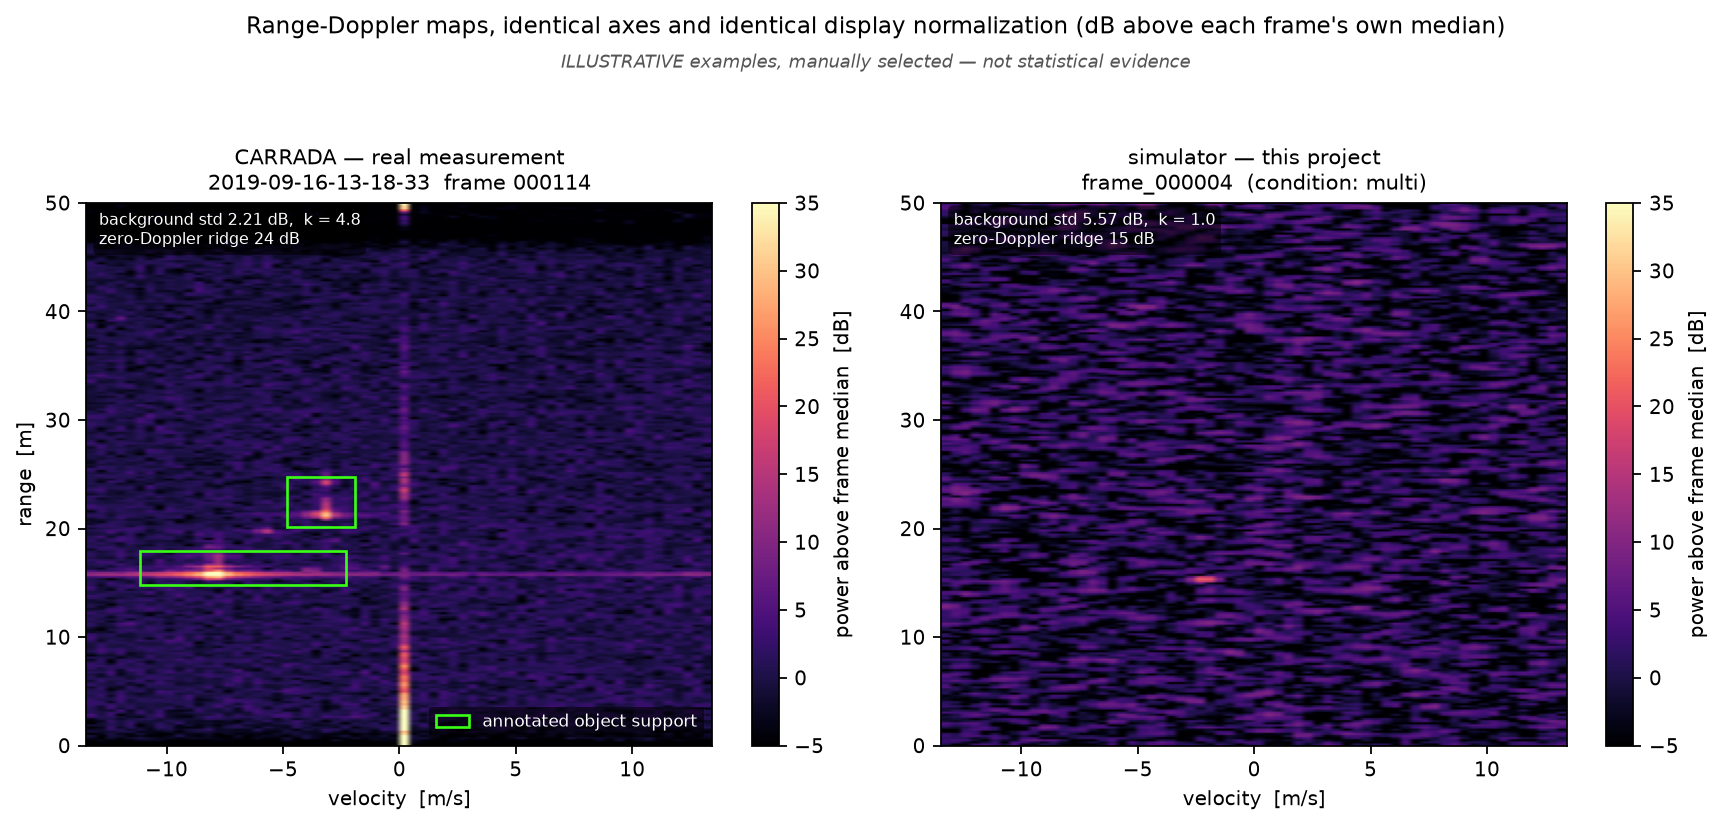
\includegraphics[width=\textwidth]{figures/Chapter7/r0_fig1_rd_examples.png}
\caption[Range--Doppler maps from the real and synthetic domains]{One range--Doppler frame from each
domain, on identical physical axes and with identical display normalisation (decibels above each
frame's own median). Left: CARRADA, with the annotated object support outlined. Right: this
project's simulator. \textbf{Illustrative examples, manually selected --- not statistical
evidence.}}
\label{fig:rd_domains}
\end{figure}

\section{Secondary findings}
\label{sec:r7secondary}

\subsection{Near range is where the two arms genuinely diverge}

Stratifying by range block is the one stratification in which the arms separate clearly, and the
pattern is not monotone. The network is behind in the nearest block --- \RoneRangeATinyCNN{} against
CA-CFAR's \RoneRangeACFAR{}, a deficit of \RoneRangeADiff{} --- and \emph{ahead} in the three middle
blocks, by as much as \RoneRangeDDiff{} at \RoneRangeDLabel{} bins. The near-range deficit is the
largest single stratified difference in the chapter, and it is consistent with the range
non-stationarity recorded in Section~\ref{sec:r7audit}: the simulator's background statistics are
stationary in range, CARRADA's are not, and the near field is where they differ most. A single
pooled number would have hidden both halves of this. Chapter~\ref{chp:domaingap} returns to the
near-range block directly, because it is the pre-specified test of whether the domain intervention
worked.

Performance near and away from the zero-Doppler ridge is similar between TinyCNN and CA-CFAR, so
the transfer difference is not concentrated there. Class-wise recall is difficult to interpret
because CARRADA classes have different annotation-mask sizes, which directly changes the area in
which a detection can count as correct. Detailed stratified results are therefore left to
Appendix~\ref{app:tables}.

\begin{quote}
\textbf{A large structural difference between domains does not translate mechanically into a
detector difference.} The audit's biggest finding --- the ridge --- shows no detector separation; the
clearest separation appears where the audit measured range non-stationarity instead.
\end{quote}

\subsection{Tolerance around the annotated support}

Since the truth is a region rather than a point, it is worth asking whether the misses fall just
outside it. Dilating the mask by $\pm 1$ and $\pm 3$ bins, identically for both arms, gives the
ladder in Table~\ref{tab:r1_tolerance}.

\begin{table}[H]
\centering
\caption{Recall with the annotated support dilated. This measures tolerance around the annotation,
\emph{not} localisation accuracy.}
\label{tab:r1_tolerance}
\begin{tabular}{@{}lccc@{}}
\toprule
\textbf{Detector} & \textbf{Exact} & \textbf{$\pm 1$ bin} & \textbf{$\pm 3$ bins} \\
\midrule
TinyCNN  & \RoneTinyCNNExact & \RoneTinyCNNTolOne & \RoneTinyCNNTolThree \\
CA-CFAR  & \RoneCFARCAExact  & \RoneCFARCATolOne  & \RoneCFARCATolThree \\
\midrule
Difference & \RoneDiffExact & \RoneDiffTolOne & \RoneDiffTolThree \\
\bottomrule
\end{tabular}
\end{table}

The network gains substantially more from dilation than the classical detector does, and the
ordering changes as the tolerance widens. A larger share of the network's misses are therefore near
misses lying just outside the annotated region. Two cautions apply. This is \textbf{not} a
localisation measurement: with extended truth there is no point against which localisation could be
measured, and dilating a mask asks whether a peak fell \emph{near} the annotated support, which is a
different question from how precisely it was placed. And a detector that emits more candidates has
more chances to land one inside a dilated region; the network emits \RoneBurdenRatio{} times
CA-CFAR's output, so part of this gain is bought rather than earned.

The same shape appears in the synthetic domain, where the frozen network gains from a wider gate and
loses at the exact cell (Section~\ref{sec:localization}). A broader detector response is consistent
with both observations and may contribute to both, but it is not established as the cause of either,
and separating response breadth from output density would need an intervention that was not
performed. The breadth itself belongs to this frozen arm's $3\times3$ block label, which
Chapter~\ref{chp:attribution} shows is largely removable, not to learned detection as such.

\subsection{Seed variability}

The eight frozen seeds span \RoneSeedMin{} to \RoneSeedMax{}, a standard deviation of
\RoneSeedSD{}; \RoneSeedsAboveCFAR{} of the eight exceed CA-CFAR's \RoneCFARCA{} and the rest fall
below it, which is what a genuinely close comparison looks like at the seed level. No seed was
selected, dropped or ensembled at any point. The spread is small in absolute terms --- comparable to
the paired difference being measured --- so the pooled result is not an average over wildly different
networks. It is not negligible either: eight networks with near-identical synthetic development
performance still differ measurably under domain shift, and a single-seed result would have been
reported as a win or a loss depending only on which seed happened to be trained. That is why every
network value in this report is a mean over \TinySeeds{} seeds. This is a property of this detector
and this training configuration, not evidence about neural networks in general.

\begin{figure}[htbp]
\centering
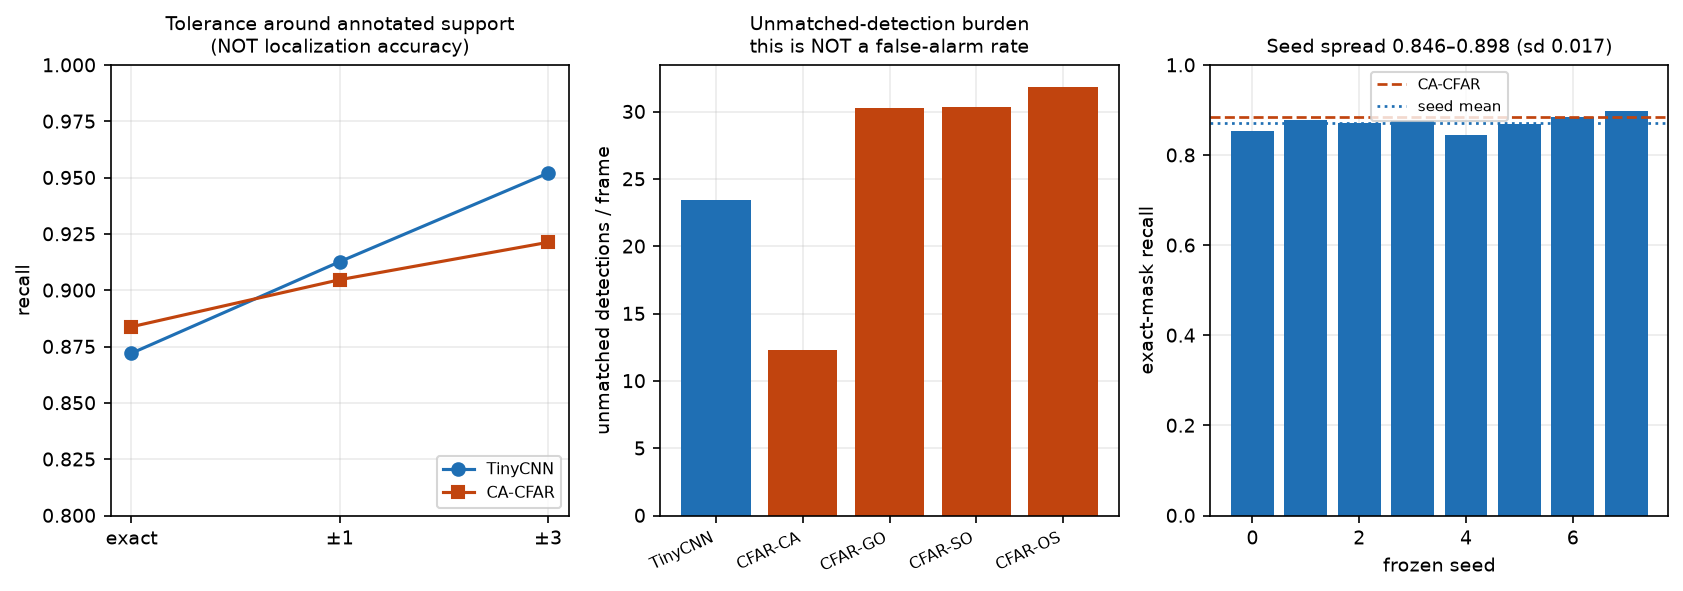
\includegraphics[width=\textwidth]{figures/Chapter7/r1_fig3_tolerance_burden_seeds.png}
\caption[Tolerance ladder, output burden and seed spread]{The three secondary findings in one view.
Left: recall against mask dilation --- the network gains more from a wider tolerance. Centre:
unmatched detections per frame, the axis on which the arms clearly differ. Right: the eight frozen
seeds against CA-CFAR's recall (dashed line).}
\label{fig:r1_tolerance}
\end{figure}

\subsection{Post-processing matters more on extended objects}

A methodological finding emerged that the chapter did not set out to make. This comparison is
sensitive not only to the two score maps but to the fixed rule converting a dense score map into
object candidates. The synthetic benchmark never exercises that sensitivity: its targets are points,
and any reasonable suppression window holds one maximum per target. Real annotated objects are
\emph{larger} than the suppression window, so the same rule operates \emph{inside} a single object,
and which local maximum survives is close to arbitrary. The ranking of two detectors on real
extended-object data therefore depends on that post-processing choice as well as on the detectors.
Appendix~\ref{app:prereg} records how this was found and what it moved.

\section{Placing the result against published work}
\label{sec:litcompare}

Section~\ref{sec:sota} separated the reviewed corpus into families and established that only one of
them --- per-cell learned thresholding scored against CFAR at a matched false-alarm rate --- measures
the same quantity as this work. Only that family is used for numerical comparison, and the purpose is
calibration, not advocacy. Table~\ref{tab:lit_regime} sets out both what each work measured and the
training regime it measured it under.

\begin{table}[H]
\centering\small
\caption{The comparable literature: reported margin over a classical baseline, and whether the
evaluation domain was represented in training.}
\label{tab:lit_regime}
\begin{tabular}{@{}p{2.6cm}p{4.1cm}p{4.2cm}p{2.6cm}@{}}
\toprule
\textbf{Work} & \textbf{Data and training} & \textbf{Reported margin} &
\textbf{Test domain seen in training?} \\
\midrule
RadCNN~\cite{yavuz2021radcnn} & Simulated pulse-Doppler, Weibull and K clutter; same simulator for
test & $+1$\,dB best case, $-0.8$\,dB worst; $P_{fa}$ matched by design & Yes \\
\addlinespace
Lallouet et al.~\cite{lallouet2023loss} & Simulated exoclutter; same simulator for test &
All network variants ahead of CFAR & Yes \\
\addlinespace
Gusland et al.~\cite{gusland2020deeptemporal} & Real X-band FMCW, trained and tested at different
locations & $+0.25$ to $+0.35$ $P_d$ at clutter transitions; parity below \SI{450}{\metre} &
Yes --- same sensor \\
\addlinespace
Banerjee et al.~\cite{banerjee2025rctd} & Simulation, plus on-air captures of a single parked
reflector & Comparable $P_d$ at lower $P_{fa}$; below \SI{80}{\percent} under interference &
Partly \\
\midrule
\textbf{This work} & \textbf{Simulation only; CARRADA test split} &
$\mathbf{+\SynSnrGainDL}$\,\textbf{dB} synthetic, at measured $P_{fa}$;
\textbf{\RoneDelta{}} zero-shot & \textbf{No --- zero-shot} \\
\bottomrule
\end{tabular}
\end{table}

Three statements are supported, and they answer the three questions this comparison can settle.

\textbf{The synthetic margin is of a normal size.} At \SynSnrGainDL{}\,dB it sits alongside
RadCNN's average of about $+0.5$\,dB, and was measured under a stricter condition: RadCNN matches
$P_{fa}$ by design and reports its CFAR arms drifting to between $1.2$ and
$1.7 \times 10^{-3}$ against a design value of $10^{-3}$, whereas the arms here are matched at
measured $P_{fa}$. The clutter-edge margin,
\SynClutterEdgeDiff{} in $P_d$, is similar in magnitude to the $+0.25$ to $+0.35$ band Gusland
et al.\ report for clutter transitions on real X-band data with a different architecture, waveform
and target class. The homogeneous-clutter tie is likewise consistent with RadCNN's noise-only
scenario and Gusland's sub-\SI{450}{\metre} regime.

\textbf{This transfer regime is not directly represented in the reviewed corpus.} No work in the
comparable family evaluates a detector on real data drawn from a domain it never saw in training.
The nearest is Banerjee et al., whose on-air data is a single parked reflector at high SNR ---
a controlled capture, not a moving street scene. Gusland et al.\ come closest in spirit, training
and testing at different physical locations, but both sets are real measurements from the same
sensor: the gap there is one of scene, not of data-generating process. \textbf{No directly
comparable zero-shot synthetic-to-real experiment was identified in the reviewed corpus}, so the
transfer result has no external benchmark against which to calibrate it, and a single measurement is
not a norm.

\textbf{The nearest supporting observation points the same way.} Tosi et
al.~\cite{tosi2025benchmarking} train a CNN peak detector on a linearised signal model, evaluate it
on data containing hardware nonlinearities, and find it comparable to CFAR within its training
regime and degrading outside it --- attributing that to the coverage of the training distribution
rather than to the architecture. That is the same failure mode, observed independently on a
different problem.

Two further points bound the reading. Every comparable work reports a condition in which its network
loses; the synthetic suite of Chapter~\ref{chp:synthetic} contains no such condition, which is more
plausibly a gap in the suite than a property of this network. RadCNN's losing scenario --- target in
noise with clutter intruding into the reference window --- has no counterpart among the seven
conditions evaluated here, and constructing one would be a direct extension of this work. And none
of these comparisons establishes that the detector built here outperforms any published detector:
the systems differ in architecture, data, waveform, metric and operating point, and the table
compares \emph{margins over a classical baseline}, not detectors.

One adjacent calibration is admissible for a single purpose. DAROD~\cite{decourt2022darod}, a
$3.4$-million-parameter detector trained on the CARRADA training split, reports a recall of
$46.03\,\%$ at an IoU threshold of $0.5$ on the same test split used here. That number is
\textbf{not} comparable with the \RoneTinyCNN{} of Table~\ref{tab:r1_primary}: DAROD's metric
requires a predicted box to overlap the annotation by a fixed fraction \emph{and} carry the correct
class label, whereas the metric here asks only whether a detected peak falls inside the annotated
support, and is by a wide margin the more permissive of the two. No ranking between the systems is
claimed. What it does establish is that CARRADA is a demanding benchmark, on which a purpose-built
supervised detector trained on the dataset itself still misses roughly half of the annotated objects
under its own criterion --- against which a simulator-trained network reaching recall comparable to a
classical detector reads as a reasonable zero-shot outcome rather than a defective one.

\section{Limitations}
\label{sec:limits}

\begin{enumerate}
\itemsep4pt

\item \textbf{Dataset scope.} CARRADA is one sensor on one test track, and the effective sample
size for inference is \RoneNseq{} test sequences. The confidence interval is wide because six
sequences is not many, and a second dataset could reinforce or overturn this result.

\item \textbf{Ground truth and metric mismatch.} The primary metric asks whether a peak lands inside
an extended annotated region. It is not the synthetic point-target $P_d$, and the two are never
pooled. Class sizes and mask extents are also unbalanced --- the most numerous class has the smallest
masks --- so per-class recall cannot be read as class difficulty alone.

\item \textbf{No false-alarm measurement exists.} The comparison is one-sided: it measures what each
detector finds, not what it invents. Unmatched detections are an output-density measure and not a
false-alarm rate. This bounds the chapter's central trade-off rather than resolving it, since the
network's larger output cannot be priced against its recall on this dataset.

\item \textbf{Post-processing and data imbalance.} The post-processing was designed for synthetic
point targets, whereas a real CARRADA object can cover many range--Doppler cells. A single object
can therefore produce several surviving peaks; after one is matched, the others contribute to the
unmatched-output count. The burden metric is therefore partly sensitive to the chosen NMS radius. In
addition, \RoneNearZeroFrac{} of test objects overlap the zero-Doppler region, so the headline
result mainly reflects performance in that part of the map.

\item \textbf{Transfer scope.} No real-data training was performed \emph{in this chapter}, so its
result is a zero-shot bound and not a ceiling. CFAR is also zero-shot here: its multipliers were
calibrated for single-look statistics, so its operating point on real data is not the designed one,
and that it transferred well is an observation rather than evidence its calibration was correct.
Finally, this chapter performs no causal intervention, so none of the measured domain differences
can be said, on its evidence alone, to have caused the result. Chapter~\ref{chp:domaingap} tests
exactly what this bound leaves open, as follow-up work carried out after this evaluation.

\end{enumerate}

\section{Conclusion}

This chapter asked whether the frozen detectors transfer zero-shot from the simulator to real
automotive radar data, and answered it under a protocol fixed in advance of the answer.

Both detectors transfer in the sense that both work: neither collapses on real measurements, and
both recall the large majority of annotated objects from a purely synthetic development process. But
the ordering established in Chapter~\ref{chp:synthetic} does not carry over. Frozen CA-CFAR reaches
\RoneCFARCA{} exact dense-mask object recall against the frozen network's \RoneTinyCNN{}, a
sequence-balanced paired difference of \RoneDelta{} whose confidence interval
$[\RoneCIlo, \RoneCIhi]$ includes zero. \textbf{At exact annotated support the two arms are
statistically indistinguishable; the synthetic advantage is neither retained nor reversed, but
absent.} And comparable recall is bought with substantially more output: \RoneBurdenTinyCNN{}
unmatched detections per frame against CA-CFAR's \RoneBurdenCFARCA{}. \textbf{The two arms are
separable on output density even where they are not separable on recall.}

The classical family as a whole deserves its due here. \textbf{On real zero-shot transfer, the
learned detector's synthetic advantage disappears. CA-CFAR provides the cleaner low-burden baseline,
while SO- and OS-CFAR achieve the highest raw recall at the cost of denser output.} The learned arm
occupies neither position: it emits roughly twice CA-CFAR's output without matching the recall of
the robust variants.

Two qualifications complete that statement. The tolerance ladder favours the network --- more of its
misses are near misses --- but that is tolerance around an annotated region rather than localisation
accuracy, and a denser output has more chances to fall inside a dilated one. And the difference is
not concentrated at zero Doppler, which the audit had identified as the largest structural
difference between the domains; the clearest stratified separation is in the nearest range block,
where the network trails by \RoneRangeADiff{}.

None of this retracts the synthetic findings of Chapters~\ref{chp:synthetic}
and~\ref{chp:attribution}. Those were controlled experiments and they remain valid within the domain
that produced them. What this chapter establishes is the boundary of that validity: the learned
detector's measured advantage was specific to its training domain and did not transfer, while a
classical detector whose threshold adapts to local statistics by construction reached comparable
recall from a far sparser output.

\textbf{That shifts the question from detector capacity to domain alignment.} The audit of
Section~\ref{sec:r7audit} was run to decide whether this comparison was fair, but it also measured
something else: the simulator and the real sensor differ in background smoothness, spread, ridge
structure and range behaviour by margins far larger than any constant tuned anywhere in this
project. A detector whose decision rule is fixed by weights fitted to one of those distributions was
never guaranteed to carry to the other. That turns a negative result into a testable hypothesis ---
that the training distribution, not the architecture, is what failed to transfer --- and it is the
hypothesis Chapter~\ref{chp:domaingap} sets out to test.
